%
% File acl2019.tex
%
%% Based on the style files for ACL 2018, NAACL 2018/19, which were
%% Based on the style files for ACL-2015, with some improvements
%%  taken from the NAACL-2016 style
%% Based on the style files for ACL-2014, which were, in turn,
%% based on ACL-2013, ACL-2012, ACL-2011, ACL-2010, ACL-IJCNLP-2009,
%% EACL-2009, IJCNLP-2008...
%% Based on the style files for EACL 2006 by 
%%e.agirre@ehu.es or Sergi.Balari@uab.es
%% and that of ACL 08 by Joakim Nivre and Noah Smith

\documentclass[11pt,a4paper]{article}
\usepackage[hyperref]{acl2019}
\usepackage{times}
\usepackage{latexsym}

\usepackage{graphicx}
\usepackage{subcaption}

\usepackage{url}

\aclfinalcopy % Uncomment this line for the final submission
%\def\aclpaperid{***} %  Enter the acl Paper ID here

%\setlength\titlebox{5cm}
% You can expand the titlebox if you need extra space
% to show all the authors. Please do not make the titlebox
% smaller than 5cm (the original size); we will check this
% in the camera-ready version and ask you to change it back.

\newcommand\BibTeX{B\textsc{ib}\TeX}

\title{Project 1 : Auto-encoders}

\author{Prakhar Singh \\
  ps32856 \And
  Prateek Chaudhry \\
  pc26978 \And
  Shivam Garg \\ sg48957}

\date{}

\begin{document}
\maketitle
\begin{abstract}
In this project, we build an autoencoder to compress images by approximately 99\% using deep convolutional neural networks. The network was trained on diverse data comprising of canonical as well as non canonical images to increase robustness.
\end{abstract}

\section{Introduction}

We tackle the problem of compressing images using a deep convolutional autoencoder. An autoencoder is a type of neural network that learns useful encodings of input data in an unsupervised manner. It consists of two parts: (i) an encoder, which maps high dimensional input to a low dimensional encoding and (ii) a decoder, which attempts to reconstruct the original input from this low dimensional encoding.

\section{Dataset}
We built our dataset by randomly sampling images from multiple sources common in computer vision literature as listed below:
\begin{itemize}
    \item ImageNet \cite{imagenet_cvpr09} - 15000 images
    \item Places2 \cite{zhou2014learning} - 15000 images
    \item LVIS \cite{Gupta_2019_CVPR} - 5000 images
    \item Labeled Faces in the Wild \cite{LFWTech} - 2500 images
\end{itemize}
These data sources were chosen so as to get a good mix of both canonical as well as non canonical images, which is critical for training a robust model.

\section{Model Architecture}

Our architecture consists of an encoder and decoder, as described in \autoref{encoder} and \autoref{decoder}. 

Our encoder is 11 layer deep network with residual connections. These layers can be grouped in terms of reducing layers and convolutional blocks. Each block has a skip connection across it. 

The decoder is structured to be a mirror of encoder architecture and follows a similar pattern.

\begin{table}[h]
\begin{center}
\begin{tabular}{|c|c|c|}
\hline \textbf{Layer} & \textbf{Output} & \textbf{Details} \\ \hline
block\_0 & 256x256x16 & 3x3, 16 \\
reduce\_0 & 128x128x16 & 3x3, 16\\
block\_1 & 128x128x16 & 
$[\begin{array}{l}
    3x3, 16 \\
    3x3, 16
  \end{array}]$\\
reduce\_1 & 64x64x16 & 3x3, 16\\
block\_2 & 64x64x16 & 
$[\begin{array}{l}
    3x3, 16 \\
    3x3, 16
  \end{array}]$\\
reduce\_2 & 32x32x16 & 3x3, 16\\
block\_3 & 32x32x16 & 
$[\begin{array}{l}
    3x3, 16 \\
    3x3, 16
  \end{array}]$\\
\hline
\end{tabular}
\end{center}
\caption{\label{encoder} Encoder Architecture }
\end{table}

\begin{table}[h]
\begin{center}
\begin{tabular}{|c|c|c|}
\hline \textbf{Layer} & \textbf{Output} & \textbf{Details} \\ \hline
expand\_0 & 32x32x16 & 3x3, 16 \\
block\_0 & 32x32x16 & 
$[\begin{array}{l}
    3x3, 16 \\
    3x3, 16
  \end{array}]$\\
  
expand\_1 & 64x64x16 & 3x3, 16 \\
block\_1 & 64x64x16 & 
$[\begin{array}{l}
    3x3, 16 \\
    3x3, 16
  \end{array}]$\\
  
expand\_2 & 128x128x16 & 3x3, 16 \\
block\_2 & 128x128x16 & 
$[\begin{array}{l}
    3x3, 16 \\
    3x3, 16
  \end{array}]$\\
  
expand\_3 & 256x256x16 & 3x3, 16 \\
block\_3 & 256x256x3 &  3x3, 3 \\
\hline
\end{tabular}
\end{center}
\caption{\label{decoder} Decoder Architecture }
\end{table}

\section{Experiments}

\begin{table}[h]
\begin{center}
\begin{tabular}{|c|c|}
\hline \textbf{Experiment} & \textbf{Result} \\ \hline
4 conv  + 4 deconv & 0.0523\\
6 conv + 6 deconv & 0.0601\\
4 conv  + 4 deconv + l2 loss & 0.0623\\
Final architecture & \textbf{0.0477}\\
\hline
\end{tabular}
\end{center}
\caption{\label{experiment} Experiments }
\end{table}
We use pytorch to build our autoencoder and minimize L1 loss. We used adam optimizer with learning rate of 1e-3 and trained for 200 epochs. For experiment purposes, we split data into 2 parts, with training set of 35000 images and remaining 2500 images as dev set. Various architectures were tried as listed in  \autoref{experiment}. The results we report are the per pixel L1 loss averaged across whole dev set, with pixel values represented as floats between 0 and 1. Finally we trained the model on the whole dataset.

\begin{figure*}[]
  \centering
  \begin{subfigure}[b]{0.4\linewidth}
    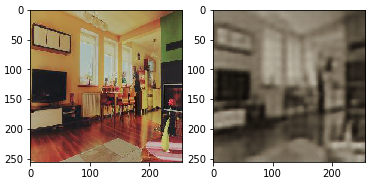
\includegraphics[width=\linewidth]{ep0.png}
    \caption{Epoch 1}
  \end{subfigure}
  \begin{subfigure}[b]{0.4\linewidth}
    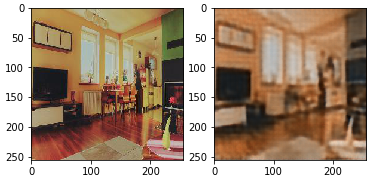
\includegraphics[width=\linewidth]{ep8.png}
    \caption{Epoch 8}
  \end{subfigure}
  \begin{subfigure}[b]{0.4\linewidth}
    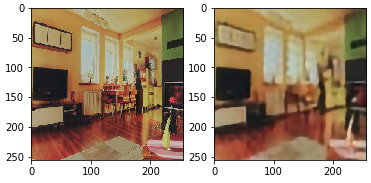
\includegraphics[width=\linewidth]{ep200.png}
    \caption{Epoch 200}
  \end{subfigure}
  \caption{Comparison of input image and reconstructed image across different training epochs}
  \label{fig:training}
\end{figure*}


In addition to loss we also looked at output images from our decoder which are shown in \autoref{fig:training}. In initial epochs, reconstructed image was quite coarse and without color. We observed color images around 8th epoch. From then on, training proceeded in a slow manner with loss slowly decreasing and finally saturating by 170th epoch.

\bibliography{acl2019}
\bibliographystyle{acl_natbib}

\end{document}
